\documentclass[letterpaper, 11pt]{article}
\usepackage[inner = 0.75in, outer = 0.75in, top = 1in, bottom = 1in, bindingoffset = 0.0 cm]{geometry}
\usepackage{amsmath}	% package to use mathematical notations
\usepackage{comment}	% package to use comment block
\usepackage{sectsty}	% to change the style of section headers
\usepackage{fancyhdr}	% to have fancy headers for each page
\usepackage{graphicx}	% allows you to import images
\usepackage{float}	% allows the control of float positions
\usepackage{makeidx} 	% to create index pages
\makeindex

% List of macros
\newcommand{\fourier}[2]{\mathcal{F}_{#1}[#2]} % Fourier transform notation
\newcommand{\fint}{\int_{-\infty}^{\infty}} % integral with infinite limits
\newcommand{\ft}[2]{\fint #2 e^{-2\pi if#1} d#1} % Fourier transform 
\newcommand{\ift}[2]{\fint #2 e^{2\pi i#1t} d#1} % Inverse Fourier transform 
\newcommand{\sed}[1]{s_{0}e^{2\pi if_{0}#1}e^{-#1/T}} % Sinusoidal exponential decay function

% Numbering equation and figure with section number
\numberwithin{equation}{section}
\numberwithin{figure}{section}

% Centering section titles
\sectionfont{\centering}

\begin{document}
% Front cover page with title and name
\begin{titlepage}
	\begin{center}
		% \vfill must have preceding text line
		\Huge{\bfseries Fourier Transform}\vfill 
	\end{center}

	\begin{flushright}
		Sejin Nam\\
		University of Hawaii at Manoa
	\end{flushright}
\end{titlepage}

\begin{comment} % commenting out standard title page
\title{Fourier Transform}
\author{Sejin Nam}
\date{May 20}
\maketitle
\thispagestyle{empty}
\clearpage
\end{comment}

% page numbering in roman numerals
\pagenumbering{roman}

% Preface
\section*{\centering Preface}
Preface text goes here
\cleardoublepage

% Table of Contents
\tableofcontents
\clearpage

% use fancyhdr
\pagestyle{fancy}

% First Section: prerequisite mathematics
\pagenumbering{arabic}
\section{Prerequisite Mathematics}
A few prerequisite mathematics will be discussed here in anticipation of their requirements in the subsequent sections after this section. 

% 1.1 Dirac Delta Function
\subsection{Dirac Delta Function}\index{Dirac Delta function}
Dirac Delta function, \(\delta (t)\), has the following property:
\begin{align}
	\delta (t)	&=\begin{cases}
		\infty, & \text{if } t = 0 \\
		0,	& \text{otherwise}
	\end{cases}\\
		1	&= \fint \delta (t) dt
\end{align}
(In my discussion of function, \(t\) variable represents time physically). The following integral is also a Dirac Delta function:
\begin{align}
	\delta (t)	&= \ift{f}{}\label{eq:dirac}
\end{align}
The above relations will be used throughout the discussion of this article.

% 1.2 Sinusoidal expoential decay function
\subsection{Sinusoidal exponential decay function}
Sinusoidal exponential decay function (I call it SED) is as follows:
\begin{equation}
	\begin{aligned}[b]
		s &= s_{0}\cos{(2\pi f_{0}t)}e^{-t/T} \theta(t)
		\label{eq:rsed}
	\end{aligned}
\end{equation}
Where \(\theta (t)\) is a Heaviside step function (the plot of such function is given in figure \ref{fig1}). You can have sine instead of cosine in the above expression. For our discussion, SED of choice is combination of sine and cosine exponential decays in complex form:
\begin{equation}
	\begin{aligned}[b]
		s	&= s_{0}\cos{(2\pi f_{0}t)}e^{-t/T} \theta(t)+ i s_{0}\sin{(2\pi f_{0}t)}e^{-t/T} \theta(t)\\
			&= (\cos{(2\pi f_{0}t)} +i \sin{(2\pi f_{0}t)})s_{0}e^{-t/T} \theta(t) \\
			&= \sed{t} \theta (t)
			\label{eq:sed}
	\end{aligned}
\end{equation}
The real part of \eqref{eq:sed} is simply \eqref{eq:rsed}.

% figure for sed function
\begin{figure}[H]
	\centering
	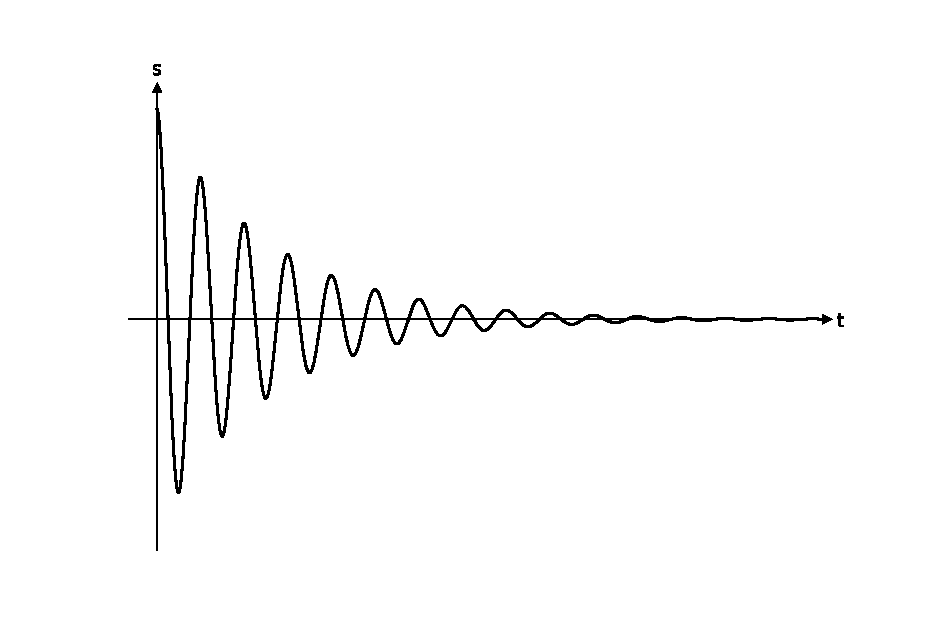
\includegraphics[height=5in]{sed.eps}
	\caption{sed function plot, s vs. t}
	\label{fig1}
\end{figure}

\clearpage

% Second Section: Fourier transform
\section{Fourier Transform}\index{Fourier transform}
Fourier transform is a mathematical transformation, in the context of my discussion, that maps one function in time domain into another function in frequency domain. There are two types of FT, Fourier transform in short: continuous and discrete. Discrete FT is of great importance in many modern data processing application as modern computers are digital, meaning they perform computation in discrete manner. I'll discuss a continous case first before moving onto the discrete case.

% 2.1 Continuous FT
\subsection{Continuous Fourier Transform}\index{Fourier transform}
Consider a continuous function of \(t\), \(x(t)\). The continuous FT of \(x\) is as follows:
\begin{equation}
	\begin{aligned}[b]
		X(f)	&=\fourier{t}{x} \\
			&=\ft{t}{x(t)}
	\end{aligned}
\end{equation}
\(X(f)\) is also continuous in \(f\) (in my discussion \(f\) represents frequency physically). You can also perform inverse FT on \(X\), which is:
\begin{equation}
	\begin{aligned}[b]
		\fourier{f}{X}	&= \ift{f}{X(f)} \\
				&= \ift{f}{\left ( \ft{\tau}{x(\tau)}\right )} \\
				&= \fint x(\tau) \fint e^{2\pi if(t - \tau)} df d\tau \\
				&= \fint x(\tau) \delta (t - \tau) d\tau \\
				&= x(t)
	\end{aligned}
\end{equation}
where I used \eqref{eq:dirac} orthogonality relation. It is easy to see that the inverse FT of one is a Dirac Delta function.

% 2.1.1 Sinusoidal exponential decay signal \subsubsection{Sinusoidal exponential decay function} Sinusoidal exponential decay (I call it SED) function is as follows:
\subsubsection{FT of SED}
The FT of SED is (with \(1/T = r\)) as follows:
\begin{equation}
	\begin{aligned}[b]
		S(f)	&= \fourier{t}{s}\\
			&= \fourier{t}{\sed{t} \theta (t)}\\
			&= s_{0}\fourier{t}{e^{-rt} \theta (t)}(f - f_{0})\\
			&= \frac{s_{0}}{r + 2\pi i(f - f_{0})} \\
			\gdef\temp{r^2 + 4\pi^{2}(f - f_{0})^2} % temporary macro
			&= s_{0}\frac{r - 2\pi i(f - f_{0})}{\temp}\\
			&= s_{0}\left[\frac{r}{\temp} + i\frac{2\pi(f_{0} - f)}{\temp} \right]
	\end{aligned}
\end{equation}
\printindex
\end{document}
